\section{Conception préliminaire}

Cette partir présente la conception préliminaire qui a été réalisée.

	\subsection{Diagramme de modèle du domaine}
	Cette partie présente les diagrammes de modèle du domaine du client et du serveur.
	Le diagramme de Modèle du Domaine serveur, sur la figure \ref{diagModeleServeur}, montre la structure envisagée pour notre serveur.
	On y trouve donc une entité Serveur chargée de la communication avec le client.
	Les autres entités représentent la structure des données pour le fonctionnement de notre application.\\
	
	Les mises à jours suite à la réalisation sont apparente sur la figure.

%TODO mettre nouveau diag
	\begin{figure}[H]
	\centerline{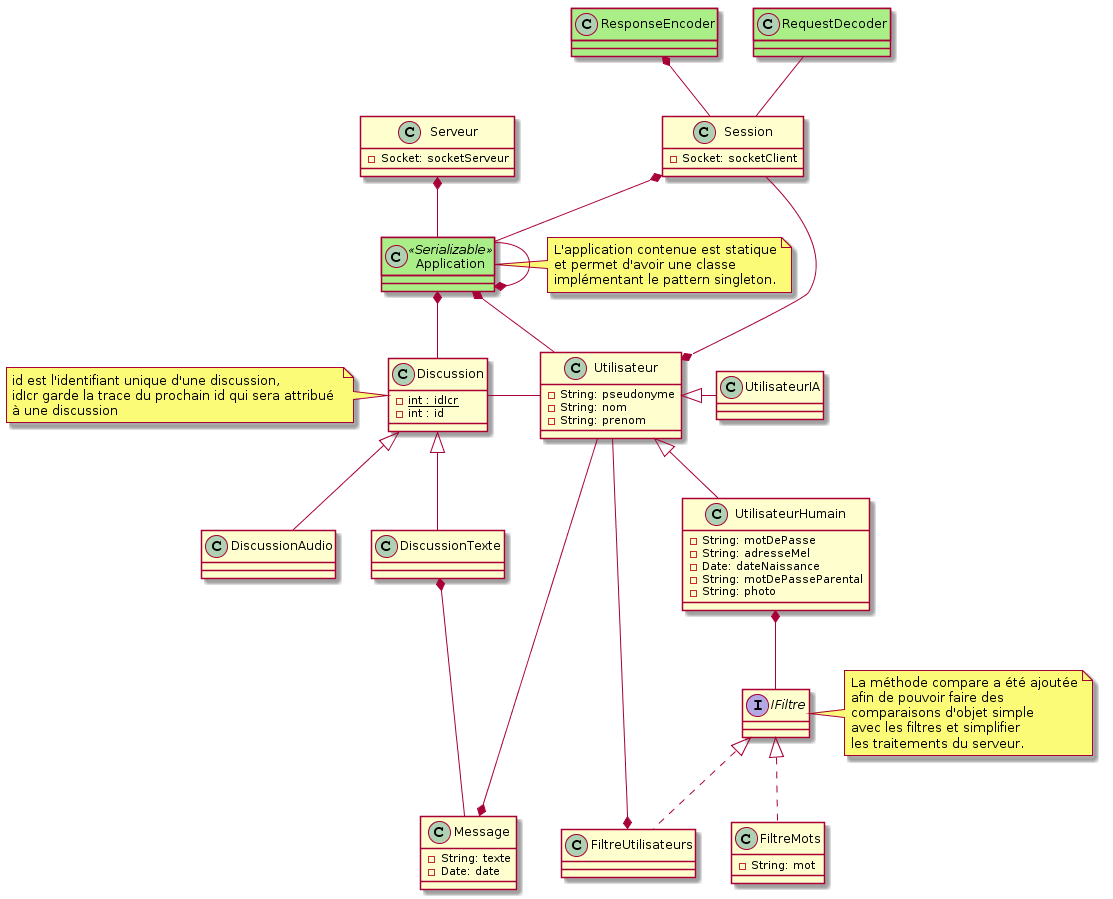
\includegraphics[width=16.5cm]{img/modeleDomaineServeurV2.png}}
	\caption{\label{diagModeleServeur}Diagramme de modèle du domaine côté serveur}
	\end{figure}

	\newpage

	Ce diagramme de Modèle du Domaine présente la structure générale de l'application du côté du client.
	Celui-ci réutilise la plupart des entités présentes dans le modèle du domaine du côté serveur.
	Ainsi, nous avons une cohérence entre les données des deux côtés. \\
	
		Les mises à jours suite à la réalisation sont apparente sur la figure \ref{modeleDomaineClient}.
		
		%TODO mettre nouveau diag
	\begin{figure}[H]
	\centerline{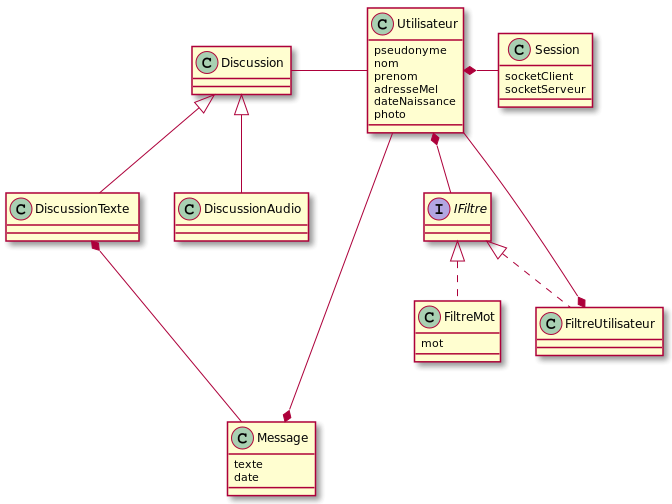
\includegraphics[width=16.5cm]{img/modeleDomaineClient.png}}
		\caption{Diagramme de modèle du domaine côté client}
		\label{modeleDomaineClient}
	\end{figure}

	\newpage

	\subsection{Diagramme de séquence système}
	
	
	Voici un diagramme séquence système correspondant au cas d'utilisation le plus important du projet : envoyer un message
	\begin{figure}[H]
		\centerline{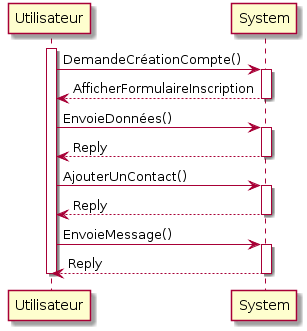
\includegraphics[width=12.5cm]{img/sequenceSystemeEnvoiMessage.png}}
		\caption{Diagramme de séquence système de l'envoi de messages}
	\end{figure}

	\newpage

	\subsection{Diagramme de navigation}
	Lorsque l'utilisateur arrive sur l'application, il arrive d'abord sur une "Page de login" où l'utilisateur a le choix entre (les champs en italique représente les modifications qui ont été effectuées) :
	\begin{itemize}
		\item connexion : entrer ses identifiants dans "Pseudonyme" et "Mot de passe" afin de se connecter en appuyant sur le bouton de validation
		\item inscription : créer un compte en cliquant sur "Pas encore inscrit ?".
		Dans ce cas, l'utilisateur arrive sur la "Page d'inscription" où il est possible d'indiquer ses identifiants "Pseudonyme", "Adresse mél", "Mot de passe", "Confirmation", "Nom", "Prénom", et "Date de naissance".
		L'utilisateur s'inscrit en appuyant sur le bouton de validation.
		L'utilisateur peut également retourner sur la "Page de connexion" en appuyant \textit{sur le bouton d'accueil}.\\
	\end{itemize}

	Lorsque l'utilisateur a passé l'étape de connexion ou d'inscription, il arrive sur la "Page de Messagerie" où il visualise les différentes conversations déjà créées. Sur cette page, différentes possibilités s'offre à lui :
	\begin{itemize}
		\item L'utilisateur peut cliquer sur une conversation déjà existante et dans ce cas il arrive sur une "Page de conversation"
		\item "Page de paramètres" : l'utilisateur peut cliquer sur l’émoticône de paramètres et dans ce cas il arrive sur la "Page de paramètres"
		\item "Page de contacts" : l'utilisateur peut cliquer sur l’émoticône des contacts, à gauche du nom de l'application, et dans ce cas il arrive sur la "Page de contacts"
		\item "Nouvelle conversation" : l'utilisateur peut cliquer sur l’émoticône "+" afin de créer une nouvelle conversation, dans ce cas une pop-up s'ouvre pour choisir un ou plusieurs utilisateurs. Il peut valider et arriver sur la "Page de conversation" associée\\
	\end{itemize}

	Lorsque l'utilisateur se situe sur une "Page de conversation", différentes possibilités s'offre à lui :
	\begin{itemize}
		\item envoyer un message en remplissant le champ et cliquer sur \textit{le bouton} envoyer
		\item "Page de paramètres" : de la même manière
		\item "Page de Messagerie" : l'utilisateur peut cliquer sur l’émoticône de \textit{Messagerie} et dans ce cas il retournera sur la "Page de Messagerie"\\
	\end{itemize}

	\newpage

	Lorsque l'utilisateur se situe sur une "Page de contacts", différentes possibilités s'offre à lui :
	\begin{itemize}
		\item appeler un contact en cliquant sur l’émoticône d'appel.
		Dans ce cas une "\textit{Page} Conversation Audio" s'ouvre, l'utilisateur pourra raccrocher en appuyant sur l’émoticône d'appel \textit{rose} afin de couper la conversation audio et retourner sur la "Page de contacts"
		\item "Page de conversation" : l'utilisateur peut cliquer sur l’émoticône de message pour contacter un contact dans une conversation privée et dans ce cas il arrive sur la "Page de Conversation" associée
		\item "Page de paramètres" : de la même manière
		\item "Page de Messagerie" : l'utilisateur peut cliquer sur l’émoticône de Messagerie, à gauche du nom de l'application, et dans ce cas il arrive sur la "Page de Messagerie"\\
	\end{itemize}

	Lorsque l'utilisateur se situe sur la "Page de paramètres", différentes possibilités s'offre à lui :
	\begin{itemize}
		\item modifier ses paramètres en remplissant les champs
		\item retourner sur la page précédente en cliquant sur l’émoticône de retour
		\item se déconnecter en cliquant sur le bouton "Déconnexion"\\
	\end{itemize}

	\begin{figure}[H]
		\centerline{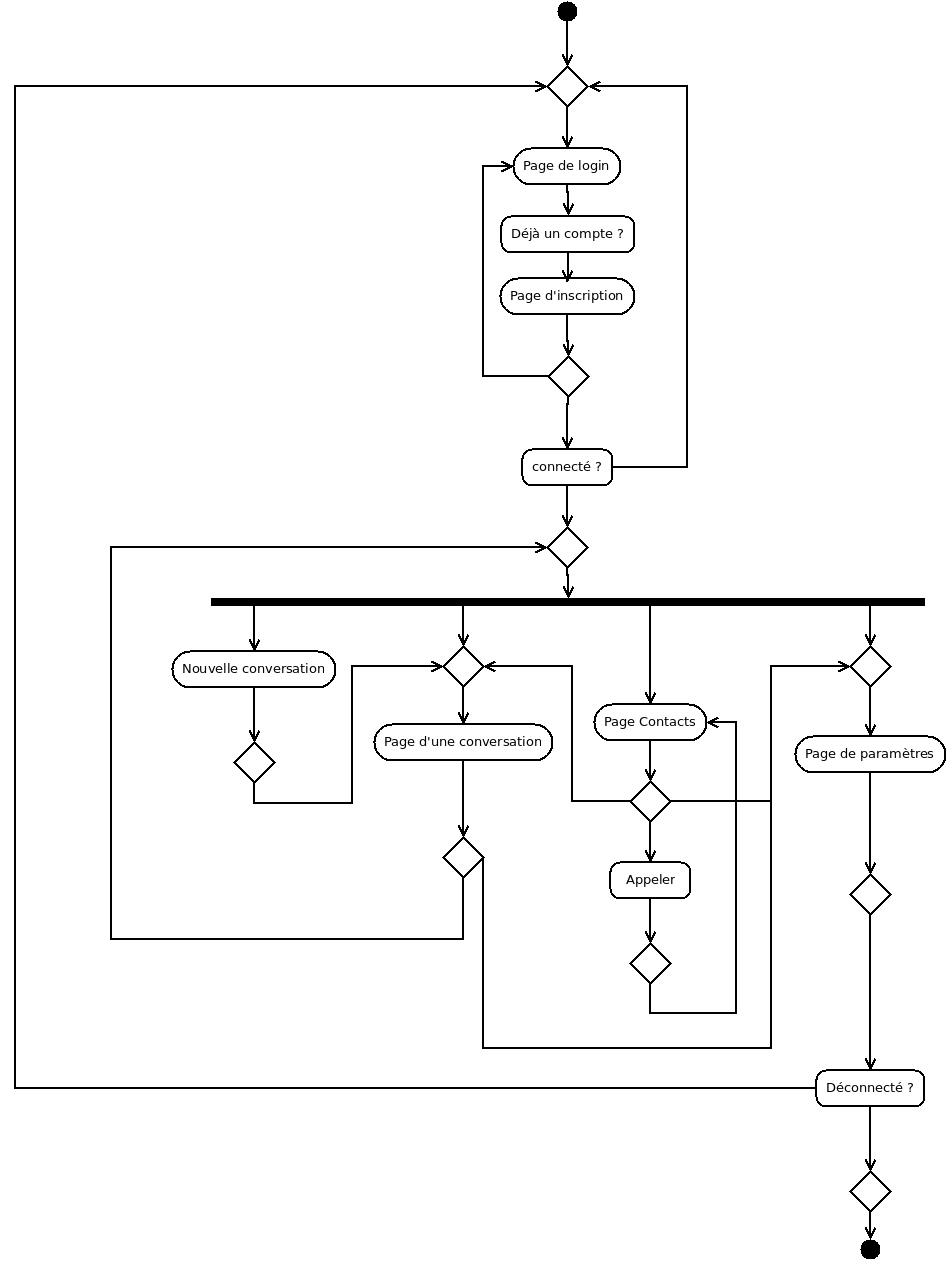
\includegraphics[width=16.5cm]{img/navigation.png}}
		\caption{Diagramme de navigation}
	\end{figure}


	\subsection{Tableau d’Interaction}
	
	Dans cette partie nous allons vous présenter toutes les interactions qui interviennent lors de l'envoi d'un message de la part d'un utilisateur à l'aide d'un tableau d’interaction et d'un diagramme d’interaction. \\

	\textbf{Tableau d’interaction pour envoyer un message :} \\

	Action de début : Vouloir envoyer un message à une personne. \\

	\begin{tabular}{|p{7cm}|p{7cm}|}
		\hline
		Action de l'utilisateur & Action du système\tabularnewline
		\hline

		\hline
		1) Entrer son login et mot de passe (A)  & \tabularnewline

		\hline
		2) Valider  & 3) Vérifier le login et le mot de passe dans la base de données\tabularnewline

		\hline
		4) Sélectionner une discussion commencée ou cliquer sur le "+" pour	démarrer une conversation avec une nouvelle personne ou aller dans les contacts et cliquer sur l’Icône message en face de la personne correspondante & \tabularnewline

		\hline
		5) Envoyer son message  & \tabularnewline
		\hline
	\end{tabular}

~\\

	Action de fin  : Message affiché dans la discussion. \\

	Exception A : Si l'utilisateur n'a pas encore de compte, la première action est de cliquer sur "Pas encore inscrit ?", ce qui envoie l'utilisateur sur la page d'inscription où il remplie le formulaire et valide.

	\begin{figure}[H]
		\centerline{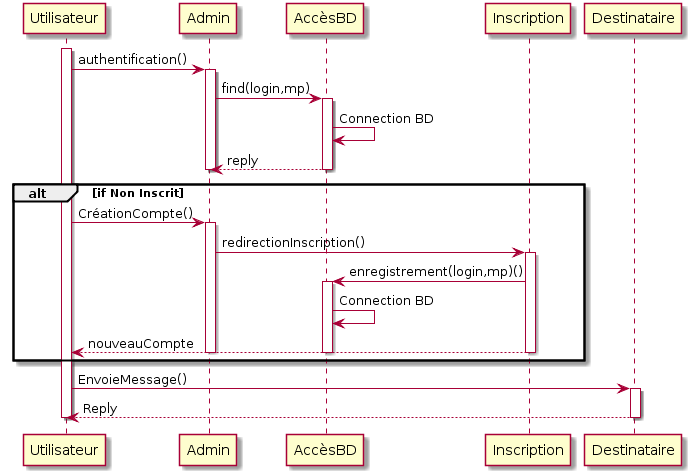
\includegraphics[width=12.5cm]{img/interaction.png}}
		\caption{Diagramme d’interaction}
	\end{figure}

	\newpage

	\subsection{Découpage en packages et signatures externes de chaque package}
	Les deux diagrammes suivants représentent le découpage en package de notre application.
	Les packages du coté serveur et client sont indépendants même si ils utilisent des classes communes puisqu'il ne sont pas dans le même langage.
	
	%TODO diag à jour ??
	\begin{figure}[H]
	\centerline{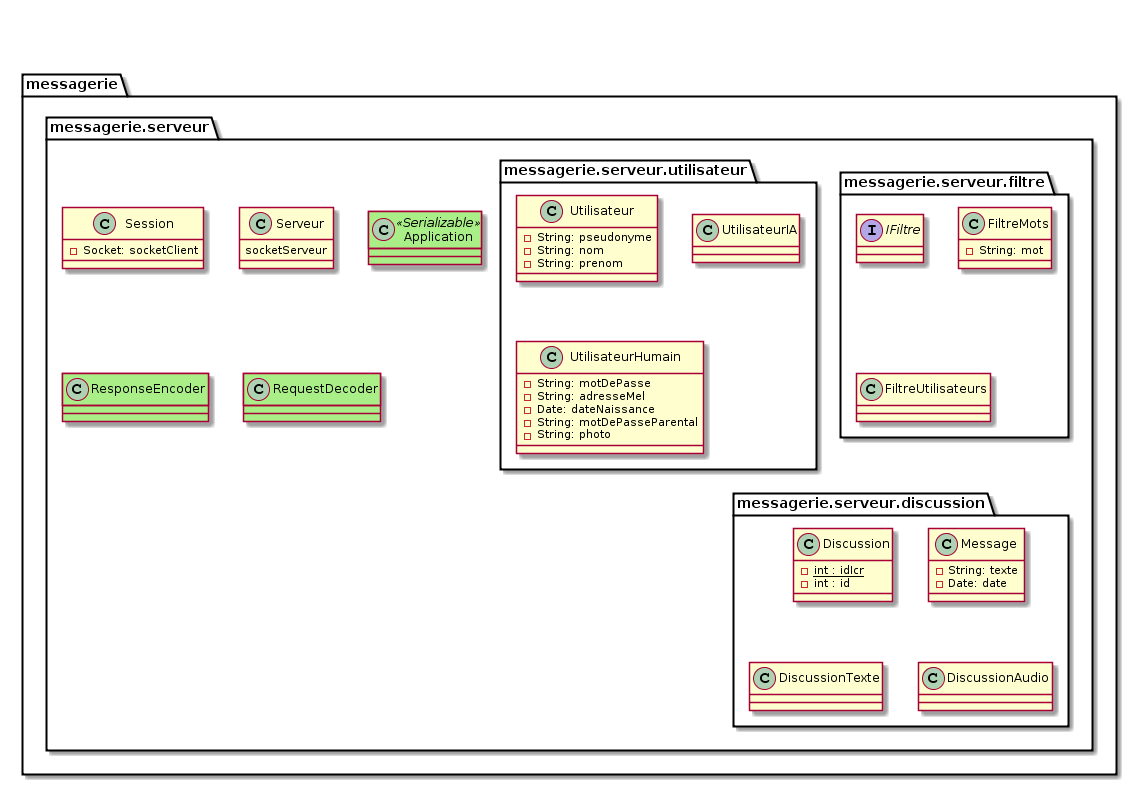
\includegraphics[width=16.5cm]{img/packageServeurV2.png}}
		\caption{Diagramme de package côté serveur}
	\end{figure}

	%TODO diag à jour ??
	\begin{figure}[H]
	\centerline{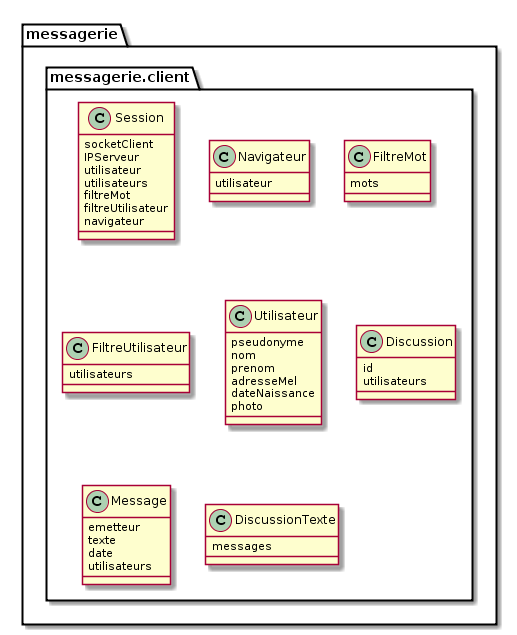
\includegraphics[width=16.5cm]{img/packageClient.png}}
	\caption{Diagramme de package côté client}
	\end{figure}